\documentclass[11pt,a4paper]{article}
\usepackage[margin=2.2cm]{geometry}
\usepackage{booktabs}
\usepackage{amsmath,amssymb}
\usepackage{mathrsfs}
\usepackage{float}
\usepackage{graphicx}
\usepackage{microtype}
\usepackage[authoryear,round]{natbib}
\usepackage[hidelinks]{hyperref}
\urlstyle{tt}
\setlength{\emergencystretch}{1.5em}
\renewcommand{\labelitemi}{$\bullet$}
\usepackage{caption}
\renewcommand{\thetable}{S\arabic{table}}
\renewcommand{\thefigure}{S\arabic{figure}}
\title{\large\bfseries Supplementary Material B\\[3pt]\normalsize Implementation details and additional results\\[3pt]
\normalsize to \emph{An Adjusted Ersatz Discrepancy for Global Sensitivity Analysis: Theory and Benchmarks}}
\author{}\date{}
% Unicode mappings for the text layer of the PDF (search, copy, text extraction):
% the glyph names of the text and math fonts, and the big delimiters and
% operators of the math extension font, which glyphtounicode.tex does not cover
\ifdefined\pdfgentounicode
  \input{glyphtounicode}
  \pdfgentounicode=1
  \def\cmexuni#1#2{\pdfglyphtounicode{#1big}{#2}\pdfglyphtounicode{#1Big}{#2}%
    \pdfglyphtounicode{#1bigg}{#2}\pdfglyphtounicode{#1Bigg}{#2}}
  \cmexuni{parenleft}{0028}\cmexuni{parenright}{0029}
  \cmexuni{bracketleft}{005B}\cmexuni{bracketright}{005D}
  \cmexuni{braceleft}{007B}\cmexuni{braceright}{007D}
  \cmexuni{floorleft}{230A}\cmexuni{floorright}{230B}
  \cmexuni{ceilingleft}{2308}\cmexuni{ceilingright}{2309}
  \cmexuni{angbracketleft}{27E8}\cmexuni{angbracketright}{27E9}
  \cmexuni{slash}{002F}\cmexuni{backslash}{005C}\cmexuni{radical}{221A}
  \pdfglyphtounicode{integraltext}{222B}\pdfglyphtounicode{integraldisplay}{222B}
  \pdfglyphtounicode{summationtext}{2211}\pdfglyphtounicode{summationdisplay}{2211}
  \pdfglyphtounicode{producttext}{220F}\pdfglyphtounicode{productdisplay}{220F}
  \pdfglyphtounicode{uniontext}{22C3}\pdfglyphtounicode{uniondisplay}{22C3}
  \pdfglyphtounicode{intersectiontext}{22C2}\pdfglyphtounicode{intersectiondisplay}{22C2}
  \pdfglyphtounicode{vextendsingle}{2223}\pdfglyphtounicode{vextenddouble}{2225}
  \pdfglyphtounicode{mapsto}{007C}% bar of \mapsto, which precedes the arrow
\fi

\begin{document}
\maketitle

\section*{B.1 Implementation}

All computations use the Python module \texttt{discrepancy.py} (version~2.0), which implements the estimators, the test functions and the designs, with NumPy, SciPy and, for the gradient-boosting surrogate of HYMOD only, scikit-learn. The scripts of the repository produce the results as follows:
\begin{itemize}\setlength{\itemsep}{0pt}
\item \texttt{reference\_indices.py}, \texttt{delta\_reference.py} and \texttt{hymod\_reference.py}: reference values of $T_i$ and $\delta_i$ (Table~\ref{tab:refs});
\item \texttt{experiments.py}: benchmark, convergence, Becker and HYMOD experiments, and the sensitivity analysis of the method;
\item \texttt{null\_distribution.py}: distribution of the adjusted ersatz under independence (Supplementary Material~A, Table~2);
\item \texttt{theory\_checks.py}: numerical steps of Supplementary Material~A;
\item \texttt{summaries.py}, \texttt{make\_tables.py} and \texttt{make\_figures.py}: tables and figures.
\end{itemize}
Every random stream is seeded, so all tables and figures are reproducible.

\paragraph{Designs.} Scrambled Sobol' points are the first $N$ points of \path{scipy.stats.qmc.Sobol} with its default scrambling, a linear matrix scramble followed by a digital shift. Maximin Latin hypercubes are the best of 20 random Latin hypercubes (\path{scipy.stats.qmc.LatinHypercube}) by minimum distance between points. Simple random samples are independent uniform points.

\paragraph{Ersatz statistics.} Algorithm~1 of the main text, with $s=\lceil N^{\alpha_g}\rceil$, $\alpha_g=1/2$, $\theta_f=1/2$, ordinal ranks (ties broken by order of appearance) and a non-cascading fill on in-grid Moore neighbourhoods. The S-ersatz uses the min-max scaled output and no fill.

\paragraph{Polynomial chaos expansion and Shapley effects.} Full total-degree bases of orthonormal Legendre polynomials on $[0,1]$ (Hermite polynomials of the standard normal inputs of the Oakley--O'Hagan function); ordinary least squares through a QR decomposition; degree $p\in\{1,\dots,10\}$ selected by the corrected leave-one-out error of Blatman and Sudret (2010) among the degrees with $N\ge2P$ and $P\le1000$ terms. Total-order indices and Shapley effects are computed from the squared coefficients of the orthonormal basis (main text, Section~2.6).

\paragraph{PAWN.} Given-data version with $n=10$ equal-width conditioning intervals on the probability scale and the maximum of the two-sample Kolmogorov--Smirnov statistics (\path{scipy.stats.ks_2samp}) between the full output sample and each conditional sub-sample.

\paragraph{Becker metafunction.} Port of \path{sensobol::metafunction} with $k_2=0.5$ and $k_3=0.2$: thirteen univariate functions (linear, quadratic, cubic, exponential, periodic, discontinuous, non-monotonic, inverse, no effect, trigonometric, large and small piecewise, oscillation), coefficients drawn from $0.7\,N(0,0.5)+0.3\,N(0,5)$, $\lceil k/2\rceil$ pairwise and $\lceil k/5\rceil$ three-way interactions (one if $k=3$). Interaction terms are evaluated row-wise for every $k$; \path{sensobol} collapses a single sampled pair or triplet to a constant, which we do not reproduce. Input distributions: uniform, normal $N(0.5,0.15)$, Beta$(8,2)$, Beta$(2,8)$, Beta$(2,0.8)$, Beta$(0.8,2)$ and logit-normal$(0,3.16)$, all truncated to $[0,1]$, or one of them drawn per input.

\paragraph{References.} $T_i$: analytical, or Jansen estimates on scrambled Sobol' designs (base size $2^{17}$ for Bratley et al. 1992, $2^{16}$ for Oakley--O'Hagan and Multiverse, $2^{13}$ for each Becker configuration); for HYMOD, Jansen estimates ($2^{15}$) on a degree-7 PCE and on a gradient-boosting surrogate of the $50{,}000$-run sample, which agree to within $0.002$ (the table reports their average). $\delta_i$: plug-in histogram estimates on $64\times64$ equiprobable cells with $N=2^{24}$ points (HYMOD: $2^{23}$ points of the PCE surrogate). Table~\ref{tab:refs} lists the values.

\begin{table}[H]\centering\small
\begin{tabular}{@{}llp{10.9cm}@{}}\toprule
Test case & Reference & Values (inputs in order)\\ \midrule
Bratley--Fox (1988) & $T_i$ & 0.278, 0.278, 0.278, 0.278, 0.278, 0.278, 0.278, 0.278\\
 & $\delta_i$ & 0.117, 0.117, 0.117, 0.117, 0.117, 0.117, 0.117, 0.117\\ \addlinespace[2pt]
Bratley et al. (1992) & $T_i$ & 0.747, 0.254, 0.082, 0.029, 0.008, 0.004, 0.001, 0.001\\
 & $\delta_i$ & 0.536, 0.178, 0.083, 0.040, 0.019, 0.012, 0.007, 0.007\\ \addlinespace[2pt]
Ishigami & $T_i$ & 0.558, 0.442, 0.244\\
 & $\delta_i$ & 0.256, 0.422, 0.201\\ \addlinespace[2pt]
Oakley--O'Hagan & $T_i$ & 0.059, 0.063, 0.036, 0.055, 0.024, 0.041, 0.058, 0.082, 0.097, 0.036, 0.151, 0.148, 0.142, 0.141, 0.155\\
 & $\delta_i$ & 0.030, 0.017, 0.030, 0.025, 0.019, 0.056, 0.056, 0.064, 0.068, 0.044, 0.119, 0.134, 0.119, 0.116, 0.129\\ \addlinespace[2pt]
Sobol' $G$ & $T_i$ & 0.787, 0.242, 0.034, 0.010, 0.000, 0.000, 0.000, 0.000\\
 & $\delta_i$ & 0.543, 0.189, 0.051, 0.028, 0.007, 0.007, 0.007, 0.007\\ \addlinespace[2pt]
Multiverse & $T_i$ & 0.130, 0.130, 0.130, 0.685, 0.113\\
 & $\delta_i$ & 0.136, 0.136, 0.136, 0.432, 0.194\\ \addlinespace[2pt]
HYMOD & $T_i$ & 0.241, 0.025, 0.403, 0.004, 0.704\\
 & $\delta_i$ & 0.215, 0.100, 0.159, 0.056, 0.332\\ \addlinespace[2pt]
\bottomrule\end{tabular}
\caption{Reference total-order indices $T_i$ and moment-independent measures $\delta_i$. The inputs of the Bratley--Fox function, and the three continuous inputs of the Multiverse function, have equal values by symmetry. The $\delta_i$ of the four non-influential inputs of the Sobol' $G$ function ($0.007$) are the residual bias of the reference estimator.}
\label{tab:refs}
\end{table}

\section*{B.2 Per-input estimates at $N=512$}

Tables~\ref{tab:in1}--\ref{tab:in7} report, for every input, the median and the inter-quartile range (in brackets) of each estimator over 100 replicates of the scrambled Sobol' design ($N=512$), and the full-sample values for HYMOD.
\begin{table}[H]\centering\footnotesize
\begin{tabular}{@{}lccccccc@{}}\toprule
Input & $T_i$ & $\delta_i$ & S-ersatz & Adj.\ ersatz & PCE & Shapley & PAWN \\ \midrule
$x_{1}$ & 0.278 & 0.117 & 0.849\,{\scriptsize[0.84,0.87]} & 0.091\,{\scriptsize[0.08,0.10]} & 0.139\,{\scriptsize[0.10,0.17]} & 0.110\,{\scriptsize[0.09,0.14]} & 0.298\,{\scriptsize[0.28,0.31]} \\
$x_{2}$ & 0.278 & 0.117 & 0.850\,{\scriptsize[0.83,0.86]} & 0.095\,{\scriptsize[0.08,0.10]} & 0.128\,{\scriptsize[0.09,0.16]} & 0.109\,{\scriptsize[0.08,0.14]} & 0.296\,{\scriptsize[0.28,0.32]} \\
$x_{3}$ & 0.278 & 0.117 & 0.849\,{\scriptsize[0.84,0.87]} & 0.092\,{\scriptsize[0.08,0.10]} & 0.160\,{\scriptsize[0.12,0.19]} & 0.133\,{\scriptsize[0.10,0.15]} & 0.298\,{\scriptsize[0.28,0.31]} \\
$x_{4}$ & 0.278 & 0.117 & 0.849\,{\scriptsize[0.83,0.87]} & 0.091\,{\scriptsize[0.08,0.10]} & 0.143\,{\scriptsize[0.12,0.18]} & 0.121\,{\scriptsize[0.10,0.15]} & 0.302\,{\scriptsize[0.29,0.32]} \\
$x_{5}$ & 0.278 & 0.117 & 0.849\,{\scriptsize[0.84,0.87]} & 0.096\,{\scriptsize[0.09,0.11]} & 0.146\,{\scriptsize[0.10,0.18]} & 0.117\,{\scriptsize[0.08,0.15]} & 0.298\,{\scriptsize[0.28,0.32]} \\
$x_{6}$ & 0.278 & 0.117 & 0.849\,{\scriptsize[0.84,0.87]} & 0.091\,{\scriptsize[0.08,0.10]} & 0.164\,{\scriptsize[0.12,0.19]} & 0.131\,{\scriptsize[0.09,0.15]} & 0.294\,{\scriptsize[0.28,0.32]} \\
$x_{7}$ & 0.278 & 0.117 & 0.847\,{\scriptsize[0.83,0.86]} & 0.093\,{\scriptsize[0.08,0.10]} & 0.138\,{\scriptsize[0.09,0.18]} & 0.118\,{\scriptsize[0.08,0.15]} & 0.300\,{\scriptsize[0.29,0.32]} \\
$x_{8}$ & 0.278 & 0.117 & 0.851\,{\scriptsize[0.84,0.87]} & 0.093\,{\scriptsize[0.08,0.11]} & 0.140\,{\scriptsize[0.10,0.19]} & 0.123\,{\scriptsize[0.09,0.16]} & 0.302\,{\scriptsize[0.29,0.32]} \\
\bottomrule\end{tabular}
\caption{Bratley--Fox (1988) product function: reference values and estimates.}
\label{tab:in1}
\end{table}
\begin{table}[H]\centering\footnotesize
\begin{tabular}{@{}lccccccc@{}}\toprule
Input & $T_i$ & $\delta_i$ & S-ersatz & Adj.\ ersatz & PCE & Shapley & PAWN \\ \midrule
$x_{1}$ & 0.747 & 0.536 & 0.618\,{\scriptsize[0.61,0.62]} & 0.474\,{\scriptsize[0.47,0.48]} & 0.747\,{\scriptsize[0.75,0.75]} & 0.704\,{\scriptsize[0.70,0.71]} & 0.827\,{\scriptsize[0.82,0.84]} \\
$x_{2}$ & 0.254 & 0.178 & 0.414\,{\scriptsize[0.41,0.42]} & 0.083\,{\scriptsize[0.08,0.09]} & 0.253\,{\scriptsize[0.25,0.25]} & 0.210\,{\scriptsize[0.21,0.21]} & 0.336\,{\scriptsize[0.32,0.35]} \\
$x_{3}$ & 0.082 & 0.083 & 0.410\,{\scriptsize[0.40,0.42]} & 0.025\,{\scriptsize[0.02,0.03]} & 0.081\,{\scriptsize[0.08,0.08]} & 0.059\,{\scriptsize[0.06,0.06]} & 0.188\,{\scriptsize[0.18,0.20]} \\
$x_{4}$ & 0.029 & 0.040 & 0.415\,{\scriptsize[0.41,0.42]} & 0.026\,{\scriptsize[0.02,0.03]} & 0.028\,{\scriptsize[0.03,0.03]} & 0.019\,{\scriptsize[0.02,0.02]} & 0.143\,{\scriptsize[0.13,0.16]} \\
$x_{5}$ & 0.008 & 0.019 & 0.414\,{\scriptsize[0.41,0.42]} & 0.023\,{\scriptsize[0.02,0.03]} & 0.008\,{\scriptsize[0.01,0.01]} & 0.005\,{\scriptsize[0.00,0.00]} & 0.116\,{\scriptsize[0.11,0.13]} \\
$x_{6}$ & 0.004 & 0.012 & 0.408\,{\scriptsize[0.40,0.41]} & 0.020\,{\scriptsize[0.01,0.03]} & 0.003\,{\scriptsize[0.00,0.00]} & 0.002\,{\scriptsize[0.00,0.00]} & 0.098\,{\scriptsize[0.09,0.11]} \\
$x_{7}$ & 0.001 & 0.007 & 0.406\,{\scriptsize[0.40,0.42]} & 0.021\,{\scriptsize[0.01,0.03]} & 0.001\,{\scriptsize[0.00,0.00]} & 0.000\,{\scriptsize[0.00,0.00]} & 0.097\,{\scriptsize[0.09,0.10]} \\
$x_{8}$ & 0.001 & 0.007 & 0.408\,{\scriptsize[0.40,0.42]} & 0.028\,{\scriptsize[0.02,0.04]} & 0.001\,{\scriptsize[0.00,0.00]} & 0.000\,{\scriptsize[0.00,0.00]} & 0.108\,{\scriptsize[0.10,0.12]} \\
\bottomrule\end{tabular}
\caption{Bratley et al. (1992) function: reference values and estimates.}
\label{tab:in2}
\end{table}
\begin{table}[H]\centering\footnotesize
\begin{tabular}{@{}lccccccc@{}}\toprule
Input & $T_i$ & $\delta_i$ & S-ersatz & Adj.\ ersatz & PCE & Shapley & PAWN \\ \midrule
$x_{1}$ & 0.558 & 0.256 & 0.596\,{\scriptsize[0.58,0.61]} & 0.223\,{\scriptsize[0.21,0.24]} & 0.558\,{\scriptsize[0.56,0.56]} & 0.436\,{\scriptsize[0.44,0.44]} & 0.337\,{\scriptsize[0.32,0.35]} \\
$x_{2}$ & 0.442 & 0.422 & 0.618\,{\scriptsize[0.61,0.63]} & 0.317\,{\scriptsize[0.30,0.33]} & 0.442\,{\scriptsize[0.44,0.44]} & 0.442\,{\scriptsize[0.44,0.44]} & 0.518\,{\scriptsize[0.51,0.53]} \\
$x_{3}$ & 0.244 & 0.201 & 0.561\,{\scriptsize[0.55,0.57]} & 0.140\,{\scriptsize[0.12,0.16]} & 0.244\,{\scriptsize[0.24,0.24]} & 0.122\,{\scriptsize[0.12,0.12]} & 0.221\,{\scriptsize[0.21,0.24]} \\
\bottomrule\end{tabular}
\caption{Ishigami function: reference values and estimates.}
\label{tab:in3}
\end{table}
\begin{table}[H]\centering\footnotesize
\begin{tabular}{@{}lccccccc@{}}\toprule
Input & $T_i$ & $\delta_i$ & S-ersatz & Adj.\ ersatz & PCE & Shapley & PAWN \\ \midrule
$x_{1}$ & 0.059 & 0.030 & 0.509\,{\scriptsize[0.49,0.53]} & 0.043\,{\scriptsize[0.04,0.05]} & 0.061\,{\scriptsize[0.06,0.06]} & 0.031\,{\scriptsize[0.03,0.03]} & 0.154\,{\scriptsize[0.14,0.17]} \\
$x_{2}$ & 0.063 & 0.017 & 0.510\,{\scriptsize[0.49,0.52]} & 0.040\,{\scriptsize[0.03,0.05]} & 0.065\,{\scriptsize[0.06,0.07]} & 0.033\,{\scriptsize[0.03,0.03]} & 0.143\,{\scriptsize[0.13,0.16]} \\
$x_{3}$ & 0.036 & 0.030 & 0.513\,{\scriptsize[0.50,0.53]} & 0.049\,{\scriptsize[0.04,0.06]} & 0.037\,{\scriptsize[0.03,0.04]} & 0.019\,{\scriptsize[0.02,0.02]} & 0.161\,{\scriptsize[0.15,0.18]} \\
$x_{4}$ & 0.055 & 0.025 & 0.509\,{\scriptsize[0.49,0.53]} & 0.040\,{\scriptsize[0.03,0.05]} & 0.057\,{\scriptsize[0.05,0.06]} & 0.030\,{\scriptsize[0.03,0.03]} & 0.144\,{\scriptsize[0.13,0.16]} \\
$x_{5}$ & 0.024 & 0.019 & 0.512\,{\scriptsize[0.49,0.53]} & 0.043\,{\scriptsize[0.03,0.05]} & 0.025\,{\scriptsize[0.02,0.03]} & 0.014\,{\scriptsize[0.01,0.02]} & 0.153\,{\scriptsize[0.14,0.17]} \\
$x_{6}$ & 0.041 & 0.056 & 0.514\,{\scriptsize[0.50,0.53]} & 0.056\,{\scriptsize[0.05,0.06]} & 0.043\,{\scriptsize[0.04,0.05]} & 0.033\,{\scriptsize[0.03,0.03]} & 0.203\,{\scriptsize[0.19,0.23]} \\
$x_{7}$ & 0.058 & 0.056 & 0.516\,{\scriptsize[0.50,0.53]} & 0.053\,{\scriptsize[0.05,0.06]} & 0.060\,{\scriptsize[0.06,0.06]} & 0.042\,{\scriptsize[0.04,0.04]} & 0.218\,{\scriptsize[0.19,0.24]} \\
$x_{8}$ & 0.082 & 0.064 & 0.512\,{\scriptsize[0.50,0.53]} & 0.057\,{\scriptsize[0.05,0.06]} & 0.085\,{\scriptsize[0.08,0.09]} & 0.055\,{\scriptsize[0.05,0.06]} & 0.203\,{\scriptsize[0.18,0.22]} \\
$x_{9}$ & 0.097 & 0.068 & 0.514\,{\scriptsize[0.50,0.53]} & 0.056\,{\scriptsize[0.05,0.06]} & 0.101\,{\scriptsize[0.10,0.10]} & 0.074\,{\scriptsize[0.07,0.08]} & 0.246\,{\scriptsize[0.22,0.27]} \\
$x_{10}$ & 0.036 & 0.044 & 0.508\,{\scriptsize[0.49,0.53]} & 0.047\,{\scriptsize[0.04,0.06]} & 0.037\,{\scriptsize[0.04,0.04]} & 0.026\,{\scriptsize[0.02,0.03]} & 0.179\,{\scriptsize[0.16,0.19]} \\
$x_{11}$ & 0.151 & 0.119 & 0.525\,{\scriptsize[0.50,0.54]} & 0.089\,{\scriptsize[0.08,0.10]} & 0.155\,{\scriptsize[0.15,0.16]} & 0.128\,{\scriptsize[0.13,0.13]} & 0.322\,{\scriptsize[0.30,0.35]} \\
$x_{12}$ & 0.148 & 0.134 & 0.528\,{\scriptsize[0.51,0.55]} & 0.105\,{\scriptsize[0.09,0.12]} & 0.150\,{\scriptsize[0.15,0.15]} & 0.143\,{\scriptsize[0.14,0.15]} & 0.334\,{\scriptsize[0.31,0.36]} \\
$x_{13}$ & 0.142 & 0.119 & 0.523\,{\scriptsize[0.51,0.54]} & 0.085\,{\scriptsize[0.08,0.10]} & 0.140\,{\scriptsize[0.14,0.14]} & 0.119\,{\scriptsize[0.12,0.12]} & 0.305\,{\scriptsize[0.29,0.33]} \\
$x_{14}$ & 0.141 & 0.116 & 0.520\,{\scriptsize[0.51,0.54]} & 0.085\,{\scriptsize[0.07,0.10]} & 0.140\,{\scriptsize[0.14,0.14]} & 0.120\,{\scriptsize[0.12,0.12]} & 0.302\,{\scriptsize[0.27,0.33]} \\
$x_{15}$ & 0.155 & 0.129 & 0.526\,{\scriptsize[0.51,0.54]} & 0.104\,{\scriptsize[0.09,0.11]} & 0.149\,{\scriptsize[0.14,0.15]} & 0.132\,{\scriptsize[0.13,0.14]} & 0.321\,{\scriptsize[0.30,0.34]} \\
\bottomrule\end{tabular}
\caption{Oakley--O'Hagan function: reference values and estimates.}
\label{tab:in4}
\end{table}
\begin{table}[H]\centering\footnotesize
\begin{tabular}{@{}lccccccc@{}}\toprule
Input & $T_i$ & $\delta_i$ & S-ersatz & Adj.\ ersatz & PCE & Shapley & PAWN \\ \midrule
$x_{1}$ & 0.787 & 0.543 & 0.650\,{\scriptsize[0.64,0.66]} & 0.495\,{\scriptsize[0.49,0.50]} & 0.769\,{\scriptsize[0.77,0.77]} & 0.769\,{\scriptsize[0.77,0.77]} & 0.725\,{\scriptsize[0.71,0.73]} \\
$x_{2}$ & 0.242 & 0.189 & 0.469\,{\scriptsize[0.46,0.48]} & 0.121\,{\scriptsize[0.11,0.13]} & 0.192\,{\scriptsize[0.19,0.19]} & 0.192\,{\scriptsize[0.19,0.19]} & 0.339\,{\scriptsize[0.33,0.35]} \\
$x_{3}$ & 0.034 & 0.051 & 0.449\,{\scriptsize[0.43,0.46]} & 0.036\,{\scriptsize[0.03,0.05]} & 0.027\,{\scriptsize[0.03,0.03]} & 0.026\,{\scriptsize[0.03,0.03]} & 0.152\,{\scriptsize[0.14,0.16]} \\
$x_{4}$ & 0.010 & 0.028 & 0.451\,{\scriptsize[0.44,0.46]} & 0.031\,{\scriptsize[0.02,0.05]} & 0.009\,{\scriptsize[0.01,0.01]} & 0.008\,{\scriptsize[0.01,0.01]} & 0.127\,{\scriptsize[0.11,0.14]} \\
$x_{5}$ & 0.000 & 0.007 & 0.446\,{\scriptsize[0.43,0.46]} & 0.023\,{\scriptsize[0.02,0.03]} & 0.001\,{\scriptsize[0.00,0.00]} & 0.001\,{\scriptsize[0.00,0.00]} & 0.101\,{\scriptsize[0.09,0.11]} \\
$x_{6}$ & 0.000 & 0.007 & 0.448\,{\scriptsize[0.44,0.46]} & 0.025\,{\scriptsize[0.02,0.04]} & 0.001\,{\scriptsize[0.00,0.00]} & 0.001\,{\scriptsize[0.00,0.00]} & 0.109\,{\scriptsize[0.10,0.12]} \\
$x_{7}$ & 0.000 & 0.007 & 0.446\,{\scriptsize[0.43,0.46]} & 0.029\,{\scriptsize[0.02,0.05]} & 0.001\,{\scriptsize[0.00,0.00]} & 0.001\,{\scriptsize[0.00,0.00]} & 0.117\,{\scriptsize[0.10,0.13]} \\
$x_{8}$ & 0.000 & 0.007 & 0.454\,{\scriptsize[0.44,0.47]} & 0.040\,{\scriptsize[0.03,0.07]} & 0.002\,{\scriptsize[0.00,0.00]} & 0.001\,{\scriptsize[0.00,0.00]} & 0.117\,{\scriptsize[0.10,0.14]} \\
\bottomrule\end{tabular}
\caption{Sobol' $G$ function: reference values and estimates.}
\label{tab:in5}
\end{table}
\begin{table}[H]\centering\footnotesize
\begin{tabular}{@{}lccccccc@{}}\toprule
Input & $T_i$ & $\delta_i$ & S-ersatz & Adj.\ ersatz & PCE & Shapley & PAWN \\ \midrule
$\theta_1$ & 0.130 & 0.136 & 0.493\,{\scriptsize[0.49,0.50]} & 0.060\,{\scriptsize[0.05,0.07]} & 0.117\,{\scriptsize[0.11,0.12]} & 0.103\,{\scriptsize[0.10,0.11]} & 0.251\,{\scriptsize[0.24,0.26]} \\
$\theta_2$ & 0.130 & 0.136 & 0.495\,{\scriptsize[0.49,0.50]} & 0.062\,{\scriptsize[0.05,0.07]} & 0.121\,{\scriptsize[0.12,0.12]} & 0.105\,{\scriptsize[0.10,0.11]} & 0.261\,{\scriptsize[0.25,0.27]} \\
$\theta_3$ & 0.130 & 0.136 & 0.497\,{\scriptsize[0.49,0.50]} & 0.064\,{\scriptsize[0.06,0.07]} & 0.124\,{\scriptsize[0.12,0.13]} & 0.105\,{\scriptsize[0.10,0.11]} & 0.256\,{\scriptsize[0.24,0.27]} \\
$\xi$ & 0.685 & 0.432 & 0.619\,{\scriptsize[0.61,0.63]} & 0.355\,{\scriptsize[0.35,0.36]} & 0.650\,{\scriptsize[0.64,0.65]} & 0.642\,{\scriptsize[0.64,0.65]} & 0.759\,{\scriptsize[0.75,0.77]} \\
$\zeta$ & 0.113 & 0.194 & 0.507\,{\scriptsize[0.50,0.51]} & 0.089\,{\scriptsize[0.08,0.10]} & 0.085\,{\scriptsize[0.08,0.09]} & 0.047\,{\scriptsize[0.04,0.05]} & 0.170\,{\scriptsize[0.16,0.19]} \\
\bottomrule\end{tabular}
\caption{Multiverse function: reference values and estimates.}
\label{tab:in6}
\end{table}
\begin{table}[H]\centering\footnotesize
\begin{tabular}{@{}lccccccc@{}}\toprule
Input & $T_i$ & $\delta_i$ & S-ersatz & Adj.\ ersatz & PCE & Shapley & PAWN \\ \midrule
Cmax & 0.241 & 0.215 & 0.821 & 0.181 & 0.241 & 0.180 & 0.530 \\
bexp & 0.025 & 0.100 & 0.816 & 0.095 & 0.025 & 0.020 & 0.181 \\
alpha & 0.403 & 0.159 & 0.826 & 0.128 & 0.403 & 0.255 & 0.219 \\
Rs & 0.004 & 0.056 & 0.808 & 0.049 & 0.004 & 0.002 & 0.100 \\
Rq & 0.704 & 0.332 & 0.856 & 0.299 & 0.703 & 0.543 & 0.528 \\
\bottomrule\end{tabular}
\caption{HYMOD (full sample of $50{,}000$ runs): reference values and estimates.}
\label{tab:in7}
\end{table}

\section*{B.3 Other designs}

Tables~\ref{tab:agree_lhs} and \ref{tab:agree_srs} repeat Table~2 of the main text for maximin Latin hypercube and simple random sampling. HYMOD is not included for the Latin hypercube design because its sample is fixed; its SRS rows use random subsets of the $50{,}000$ runs.

\begin{table}[H]\centering\footnotesize
\begin{tabular}{@{}llccccc@{}}\toprule
Test case & Metric & S-ersatz & Adj.\ ersatz & PCE & Shapley & PAWN \\ \midrule
Bratley--Fox (1988) & $\rho_T$ & -- & -- & -- & -- & -- \\
 & MAE$_T$ & 0.579 & 0.178 & 0.125 & 0.153 & \textbf{0.043} \\
 & $\rho_\delta$ & -- & -- & -- & -- & -- \\
 & MAE$_\delta$ & 0.740 & \textbf{0.021} & 0.053 & 0.034 & 0.199 \\
\addlinespace[2pt]
Bratley et al. (1992) & $\rho_T$ & 0.86 & 0.91 & \textbf{1.00} & \textbf{1.00} & 0.93 \\
 & MAE$_T$ & 0.344 & 0.073 & \textbf{0.001} & 0.016 & 0.149 \\
 & $\rho_\delta$ & 0.85 & 0.91 & \textbf{1.00} & \textbf{1.00} & 0.93 \\
 & MAE$_\delta$ & 0.346 & \textbf{0.033} & 0.042 & 0.035 & 0.180 \\
\addlinespace[2pt]
Ishigami & $\rho_T$ & 0.14 & 0.14 & \textbf{1.00} & 0.14 & 0.14 \\
 & MAE$_T$ & 0.183 & 0.175 & \textbf{0.001} & 0.082 & 0.100 \\
 & $\rho_\delta$ & \textbf{1.00} & \textbf{1.00} & 0.14 & \textbf{1.00} & \textbf{1.00} \\
 & MAE$_\delta$ & 0.305 & \textbf{0.054} & 0.122 & 0.093 & 0.099 \\
\addlinespace[2pt]
Oakley--O'Hagan & $\rho_T$ & 0.54 & 0.68 & \textbf{0.91} & 0.84 & 0.69 \\
 & MAE$_T$ & 0.428 & 0.028 & \textbf{0.005} & 0.019 & 0.156 \\
 & $\rho_\delta$ & 0.61 & 0.74 & 0.79 & \textbf{0.95} & 0.74 \\
 & MAE$_\delta$ & 0.446 & 0.021 & 0.021 & \textbf{0.010} & 0.173 \\
\addlinespace[2pt]
Sobol' $G$ & $\rho_T$ & 0.86 & 0.91 & \textbf{0.99} & \textbf{0.99} & 0.91 \\
 & MAE$_T$ & 0.387 & 0.075 & \textbf{0.012} & \textbf{0.011} & 0.151 \\
 & $\rho_\delta$ & 0.84 & 0.89 & \textbf{0.97} & \textbf{0.97} & 0.90 \\
 & MAE$_\delta$ & 0.384 & \textbf{0.032} & 0.037 & 0.037 & 0.165 \\
\addlinespace[2pt]
Multiverse & $\rho_T$ & 0.79 & 0.67 & \textbf{0.93} & \textbf{0.93} & \textbf{0.93} \\
 & MAE$_T$ & 0.322 & 0.086 & \textbf{0.020} & 0.037 & 0.135 \\
 & $\rho_\delta$ & 0.82 & \textbf{0.97} & 0.64 & 0.64 & 0.64 \\
 & MAE$_\delta$ & 0.330 & \textbf{0.052} & 0.075 & 0.089 & 0.166 \\
\addlinespace[2pt]
Becker ensemble & $\rho_T$ & 0.87 & 0.92 & \textbf{0.98} & \textbf{0.98} & 0.93 \\
 & MAE$_T$ & 0.401 & 0.070 & \textbf{0.012} & 0.013 & 0.174 \\
\bottomrule\end{tabular}
\caption{Agreement with $T_i$ and $\delta_i$ at $N=512$, maximin Latin hypercube design (medians over 100 replicates).}
\label{tab:agree_lhs}
\end{table}

\begin{table}[H]\centering\footnotesize
\begin{tabular}{@{}llccccc@{}}\toprule
Test case & Metric & S-ersatz & Adj.\ ersatz & PCE & Shapley & PAWN \\ \midrule
Bratley--Fox (1988) & $\rho_T$ & -- & -- & -- & -- & -- \\
 & MAE$_T$ & 0.579 & 0.171 & 0.128 & 0.153 & \textbf{0.043} \\
 & $\rho_\delta$ & -- & -- & -- & -- & -- \\
 & MAE$_\delta$ & 0.739 & \textbf{0.018} & 0.053 & 0.036 & 0.198 \\
\addlinespace[2pt]
Bratley et al. (1992) & $\rho_T$ & 0.90 & 0.91 & \textbf{1.00} & \textbf{1.00} & 0.93 \\
 & MAE$_T$ & 0.350 & 0.078 & \textbf{0.001} & 0.016 & 0.152 \\
 & $\rho_\delta$ & 0.90 & 0.91 & \textbf{1.00} & \textbf{1.00} & 0.93 \\
 & MAE$_\delta$ & 0.353 & 0.036 & 0.042 & \textbf{0.035} & 0.183 \\
\addlinespace[2pt]
Ishigami & $\rho_T$ & 0.14 & 0.14 & \textbf{1.00} & 0.14 & 0.14 \\
 & MAE$_T$ & 0.191 & 0.169 & \textbf{0.001} & 0.081 & 0.106 \\
 & $\rho_\delta$ & \textbf{1.00} & \textbf{1.00} & 0.14 & \textbf{1.00} & \textbf{1.00} \\
 & MAE$_\delta$ & 0.313 & \textbf{0.050} & 0.122 & 0.093 & 0.094 \\
\addlinespace[2pt]
Oakley--O'Hagan & $\rho_T$ & 0.56 & 0.69 & \textbf{0.88} & 0.82 & 0.69 \\
 & MAE$_T$ & 0.433 & 0.026 & \textbf{0.005} & 0.019 & 0.159 \\
 & $\rho_\delta$ & 0.62 & 0.74 & 0.77 & \textbf{0.95} & 0.75 \\
 & MAE$_\delta$ & 0.450 & 0.023 & 0.021 & \textbf{0.010} & 0.176 \\
\addlinespace[2pt]
Sobol' $G$ & $\rho_T$ & 0.84 & 0.91 & \textbf{0.99} & \textbf{0.99} & 0.89 \\
 & MAE$_T$ & 0.389 & 0.081 & \textbf{0.012} & \textbf{0.012} & 0.151 \\
 & $\rho_\delta$ & 0.83 & 0.91 & \textbf{0.97} & \textbf{0.97} & 0.88 \\
 & MAE$_\delta$ & 0.388 & 0.037 & \textbf{0.036} & 0.036 & 0.168 \\
\addlinespace[2pt]
Multiverse & $\rho_T$ & 0.79 & 0.67 & \textbf{0.93} & \textbf{0.93} & \textbf{0.93} \\
 & MAE$_T$ & 0.326 & 0.082 & \textbf{0.020} & 0.037 & 0.136 \\
 & $\rho_\delta$ & 0.81 & \textbf{0.97} & 0.64 & 0.64 & 0.64 \\
 & MAE$_\delta$ & 0.336 & \textbf{0.044} & 0.072 & 0.088 & 0.170 \\
\addlinespace[2pt]
HYMOD & $\rho_T$ & 0.91 & 0.91 & \textbf{1.00} & \textbf{1.00} & 0.81 \\
 & MAE$_T$ & 0.475 & 0.173 & \textbf{0.005} & 0.075 & 0.199 \\
 & $\rho_\delta$ & 0.96 & \textbf{1.00} & 0.91 & 0.91 & 0.96 \\
 & MAE$_\delta$ & 0.578 & \textbf{0.025} & 0.151 & 0.096 & 0.202 \\
\addlinespace[2pt]
Becker ensemble & $\rho_T$ & 0.87 & 0.91 & \textbf{0.98} & \textbf{0.98} & 0.91 \\
 & MAE$_T$ & 0.404 & 0.075 & \textbf{0.013} & 0.013 & 0.175 \\
\bottomrule\end{tabular}
\caption{Agreement with $T_i$ and $\delta_i$ at $N=512$, simple random sampling (medians over 100 replicates; HYMOD: 100 random subsets).}
\label{tab:agree_srs}
\end{table}

\section*{B.4 Screening errors}

\begin{table}[H]\centering\footnotesize
\begin{tabular}{@{}llccccc@{}}\toprule
Test case & $\theta$ & S-ersatz & Adj.\ ersatz & PCE & Shapley & PAWN \\ \midrule
Bratley--Fox (1988) & 0.01 & --/0.00 & --/0.00 & --/0.00 & --/0.00 & --/0.00 \\
 & 0.05 & --/0.00 & --/0.00 & --/0.00 & --/0.00 & --/0.00 \\
 & 0.10 & --/0.00 & --/0.62 & --/0.12 & --/0.25 & --/0.00 \\
\addlinespace[2pt]
Bratley et al. (1992) & 0.01 & 1.00/0.00 & 1.00/0.00 & 0.00/0.00 & 0.00/0.00 & 1.00/0.00 \\
 & 0.05 & 1.00/0.00 & 0.00/0.33 & 0.00/0.00 & 0.00/0.00 & 1.00/0.00 \\
 & 0.10 & 1.00/0.00 & 0.00/0.50 & 0.00/0.00 & 0.00/0.00 & 0.83/0.00 \\
\addlinespace[2pt]
Ishigami & 0.01 & --/0.00 & --/0.00 & --/0.00 & --/0.00 & --/0.00 \\
 & 0.05 & --/0.00 & --/0.00 & --/0.00 & --/0.00 & --/0.00 \\
 & 0.10 & --/0.00 & --/0.00 & --/0.00 & --/0.00 & --/0.00 \\
\addlinespace[2pt]
Oakley--O'Hagan & 0.01 & --/0.00 & --/0.00 & --/0.00 & --/0.00 & --/0.00 \\
 & 0.05 & 1.00/0.00 & 0.50/0.27 & 0.00/0.00 & 0.00/0.36 & 1.00/0.00 \\
 & 0.10 & 1.00/0.00 & 0.00/0.60 & 0.10/0.00 & 0.00/0.00 & 1.00/0.00 \\
\addlinespace[2pt]
Sobol' $G$ & 0.01 & 1.00/0.00 & 1.00/0.00 & 0.00/0.25 & 0.00/0.25 & 1.00/0.00 \\
 & 0.05 & 1.00/0.00 & 0.17/0.00 & 0.00/0.00 & 0.00/0.00 & 1.00/0.00 \\
 & 0.10 & 1.00/0.00 & 0.00/0.00 & 0.00/0.00 & 0.00/0.00 & 0.83/0.00 \\
\addlinespace[2pt]
Multiverse & 0.01 & --/0.00 & --/0.00 & --/0.00 & --/0.00 & --/0.00 \\
 & 0.05 & --/0.00 & --/0.00 & --/0.00 & --/0.20 & --/0.00 \\
 & 0.10 & --/0.00 & --/0.80 & --/0.20 & --/0.40 & --/0.00 \\
\addlinespace[2pt]
HYMOD & 0.01 & 1.00/0.00 & 1.00/0.00 & 0.00/0.00 & 0.00/0.00 & 1.00/0.00 \\
 & 0.05 & 1.00/0.00 & 0.50/0.00 & 0.00/0.00 & 0.00/0.00 & 1.00/0.00 \\
 & 0.10 & 1.00/0.00 & 0.00/0.00 & 0.00/0.00 & 0.00/0.00 & 1.00/0.00 \\
\addlinespace[2pt]
Becker ensemble & 0.01 & 1.00/0.00 & 0.91/0.01 & 0.07/0.07 & 0.04/0.09 & 1.00/0.00 \\
 & 0.05 & 1.00/0.00 & 0.23/0.07 & 0.02/0.08 & 0.02/0.10 & 1.00/0.00 \\
 & 0.10 & 1.00/0.00 & 0.04/0.15 & 0.02/0.08 & 0.02/0.09 & 0.86/0.00 \\
\bottomrule\end{tabular}
\caption{Screening errors $\alpha(\theta)/\beta(\theta)$, scrambled Sobol' design ($N=512$; medians over 100 replicates; Becker ensemble: means over 512 configurations). A dash marks an undefined error (no input on that side of the threshold).}
\label{tab:scr_sobol}
\end{table}

\begin{table}[H]\centering\footnotesize
\begin{tabular}{@{}llccccc@{}}\toprule
Test case & $\theta$ & S-ersatz & Adj.\ ersatz & PCE & Shapley & PAWN \\ \midrule
Bratley--Fox (1988) & 0.01 & --/0.00 & --/0.00 & --/0.00 & --/0.00 & --/0.00 \\
 & 0.05 & --/0.00 & --/0.00 & --/0.00 & --/0.00 & --/0.00 \\
 & 0.10 & --/0.00 & --/0.50 & --/0.12 & --/0.25 & --/0.00 \\
\addlinespace[2pt]
Bratley et al. (1992) & 0.01 & 1.00/0.00 & 1.00/0.00 & 0.00/0.00 & 0.00/0.00 & 1.00/0.00 \\
 & 0.05 & 1.00/0.00 & 0.40/0.00 & 0.00/0.00 & 0.00/0.00 & 1.00/0.00 \\
 & 0.10 & 1.00/0.00 & 0.00/0.00 & 0.00/0.00 & 0.00/0.00 & 1.00/0.00 \\
\addlinespace[2pt]
Ishigami & 0.01 & --/0.00 & --/0.00 & --/0.00 & --/0.00 & --/0.00 \\
 & 0.05 & --/0.00 & --/0.00 & --/0.00 & --/0.00 & --/0.00 \\
 & 0.10 & --/0.00 & --/0.00 & --/0.00 & --/0.00 & --/0.00 \\
\addlinespace[2pt]
Oakley--O'Hagan & 0.01 & --/0.00 & --/0.00 & --/0.00 & --/0.00 & --/0.00 \\
 & 0.05 & 1.00/0.00 & 0.50/0.27 & 0.00/0.00 & 0.00/0.36 & 1.00/0.00 \\
 & 0.10 & 1.00/0.00 & 0.00/0.40 & 0.00/0.00 & 0.00/0.00 & 1.00/0.00 \\
\addlinespace[2pt]
Sobol' $G$ & 0.01 & 1.00/0.00 & 1.00/0.00 & 0.00/0.25 & 0.00/0.25 & 1.00/0.00 \\
 & 0.05 & 1.00/0.00 & 0.33/0.00 & 0.00/0.00 & 0.00/0.00 & 1.00/0.00 \\
 & 0.10 & 1.00/0.00 & 0.00/0.00 & 0.00/0.00 & 0.00/0.00 & 1.00/0.00 \\
\addlinespace[2pt]
Multiverse & 0.01 & --/0.00 & --/0.00 & --/0.00 & --/0.00 & --/0.00 \\
 & 0.05 & --/0.00 & --/0.00 & --/0.00 & --/0.20 & --/0.00 \\
 & 0.10 & --/0.00 & --/0.40 & --/0.20 & --/0.40 & --/0.00 \\
\addlinespace[2pt]
Becker ensemble & 0.01 & 1.00/0.00 & 0.98/0.00 & 0.17/0.07 & 0.10/0.08 & 1.00/0.00 \\
 & 0.05 & 1.00/0.00 & 0.48/0.03 & 0.03/0.08 & 0.03/0.09 & 1.00/0.00 \\
 & 0.10 & 1.00/0.00 & 0.08/0.11 & 0.02/0.08 & 0.02/0.10 & 0.98/0.00 \\
\bottomrule\end{tabular}
\caption{Screening errors $\alpha(\theta)/\beta(\theta)$, maximin Latin hypercube design.}
\label{tab:scr_lhs}
\end{table}

\begin{table}[H]\centering\footnotesize
\begin{tabular}{@{}llccccc@{}}\toprule
Test case & $\theta$ & S-ersatz & Adj.\ ersatz & PCE & Shapley & PAWN \\ \midrule
Bratley--Fox (1988) & 0.01 & --/0.00 & --/0.00 & --/0.00 & --/0.00 & --/0.00 \\
 & 0.05 & --/0.00 & --/0.00 & --/0.00 & --/0.00 & --/0.00 \\
 & 0.10 & --/0.00 & --/0.38 & --/0.12 & --/0.38 & --/0.00 \\
\addlinespace[2pt]
Bratley et al. (1992) & 0.01 & 1.00/0.00 & 1.00/0.00 & 0.00/0.00 & 0.00/0.00 & 1.00/0.00 \\
 & 0.05 & 1.00/0.00 & 0.60/0.00 & 0.00/0.00 & 0.00/0.00 & 1.00/0.00 \\
 & 0.10 & 1.00/0.00 & 0.00/0.00 & 0.00/0.00 & 0.00/0.00 & 1.00/0.00 \\
\addlinespace[2pt]
Ishigami & 0.01 & --/0.00 & --/0.00 & --/0.00 & --/0.00 & --/0.00 \\
 & 0.05 & --/0.00 & --/0.00 & --/0.00 & --/0.00 & --/0.00 \\
 & 0.10 & --/0.00 & --/0.00 & --/0.00 & --/0.00 & --/0.00 \\
\addlinespace[2pt]
Oakley--O'Hagan & 0.01 & --/0.00 & --/0.00 & --/0.00 & --/0.00 & --/0.00 \\
 & 0.05 & 1.00/0.00 & 0.75/0.09 & 0.00/0.00 & 0.00/0.36 & 1.00/0.00 \\
 & 0.10 & 1.00/0.00 & 0.00/0.40 & 0.00/0.00 & 0.00/0.00 & 1.00/0.00 \\
\addlinespace[2pt]
Sobol' $G$ & 0.01 & 1.00/0.00 & 1.00/0.00 & 0.00/0.00 & 0.00/0.25 & 1.00/0.00 \\
 & 0.05 & 1.00/0.00 & 0.67/0.00 & 0.00/0.00 & 0.00/0.00 & 1.00/0.00 \\
 & 0.10 & 1.00/0.00 & 0.00/0.00 & 0.00/0.00 & 0.00/0.00 & 1.00/0.00 \\
\addlinespace[2pt]
Multiverse & 0.01 & --/0.00 & --/0.00 & --/0.00 & --/0.00 & --/0.00 \\
 & 0.05 & --/0.00 & --/0.00 & --/0.00 & --/0.20 & --/0.00 \\
 & 0.10 & --/0.00 & --/0.20 & --/0.20 & --/0.40 & --/0.00 \\
\addlinespace[2pt]
HYMOD & 0.01 & 1.00/0.00 & 1.00/0.00 & 0.00/0.00 & 0.00/0.00 & 1.00/0.00 \\
 & 0.05 & 1.00/0.00 & 1.00/0.00 & 0.00/0.00 & 0.00/0.00 & 1.00/0.00 \\
 & 0.10 & 1.00/0.00 & 0.50/0.00 & 0.00/0.00 & 0.00/0.00 & 1.00/0.00 \\
\addlinespace[2pt]
Becker ensemble & 0.01 & 1.00/0.00 & 0.99/0.00 & 0.14/0.07 & 0.09/0.09 & 1.00/0.00 \\
 & 0.05 & 1.00/0.00 & 0.69/0.01 & 0.03/0.08 & 0.02/0.09 & 1.00/0.00 \\
 & 0.10 & 1.00/0.00 & 0.12/0.08 & 0.02/0.08 & 0.02/0.10 & 0.98/0.00 \\
\bottomrule\end{tabular}
\caption{Screening errors $\alpha(\theta)/\beta(\theta)$, simple random sampling.}
\label{tab:scr_srs}
\end{table}

\section*{B.5 Convergence under simple random sampling}

\begin{figure}[H]
\centering
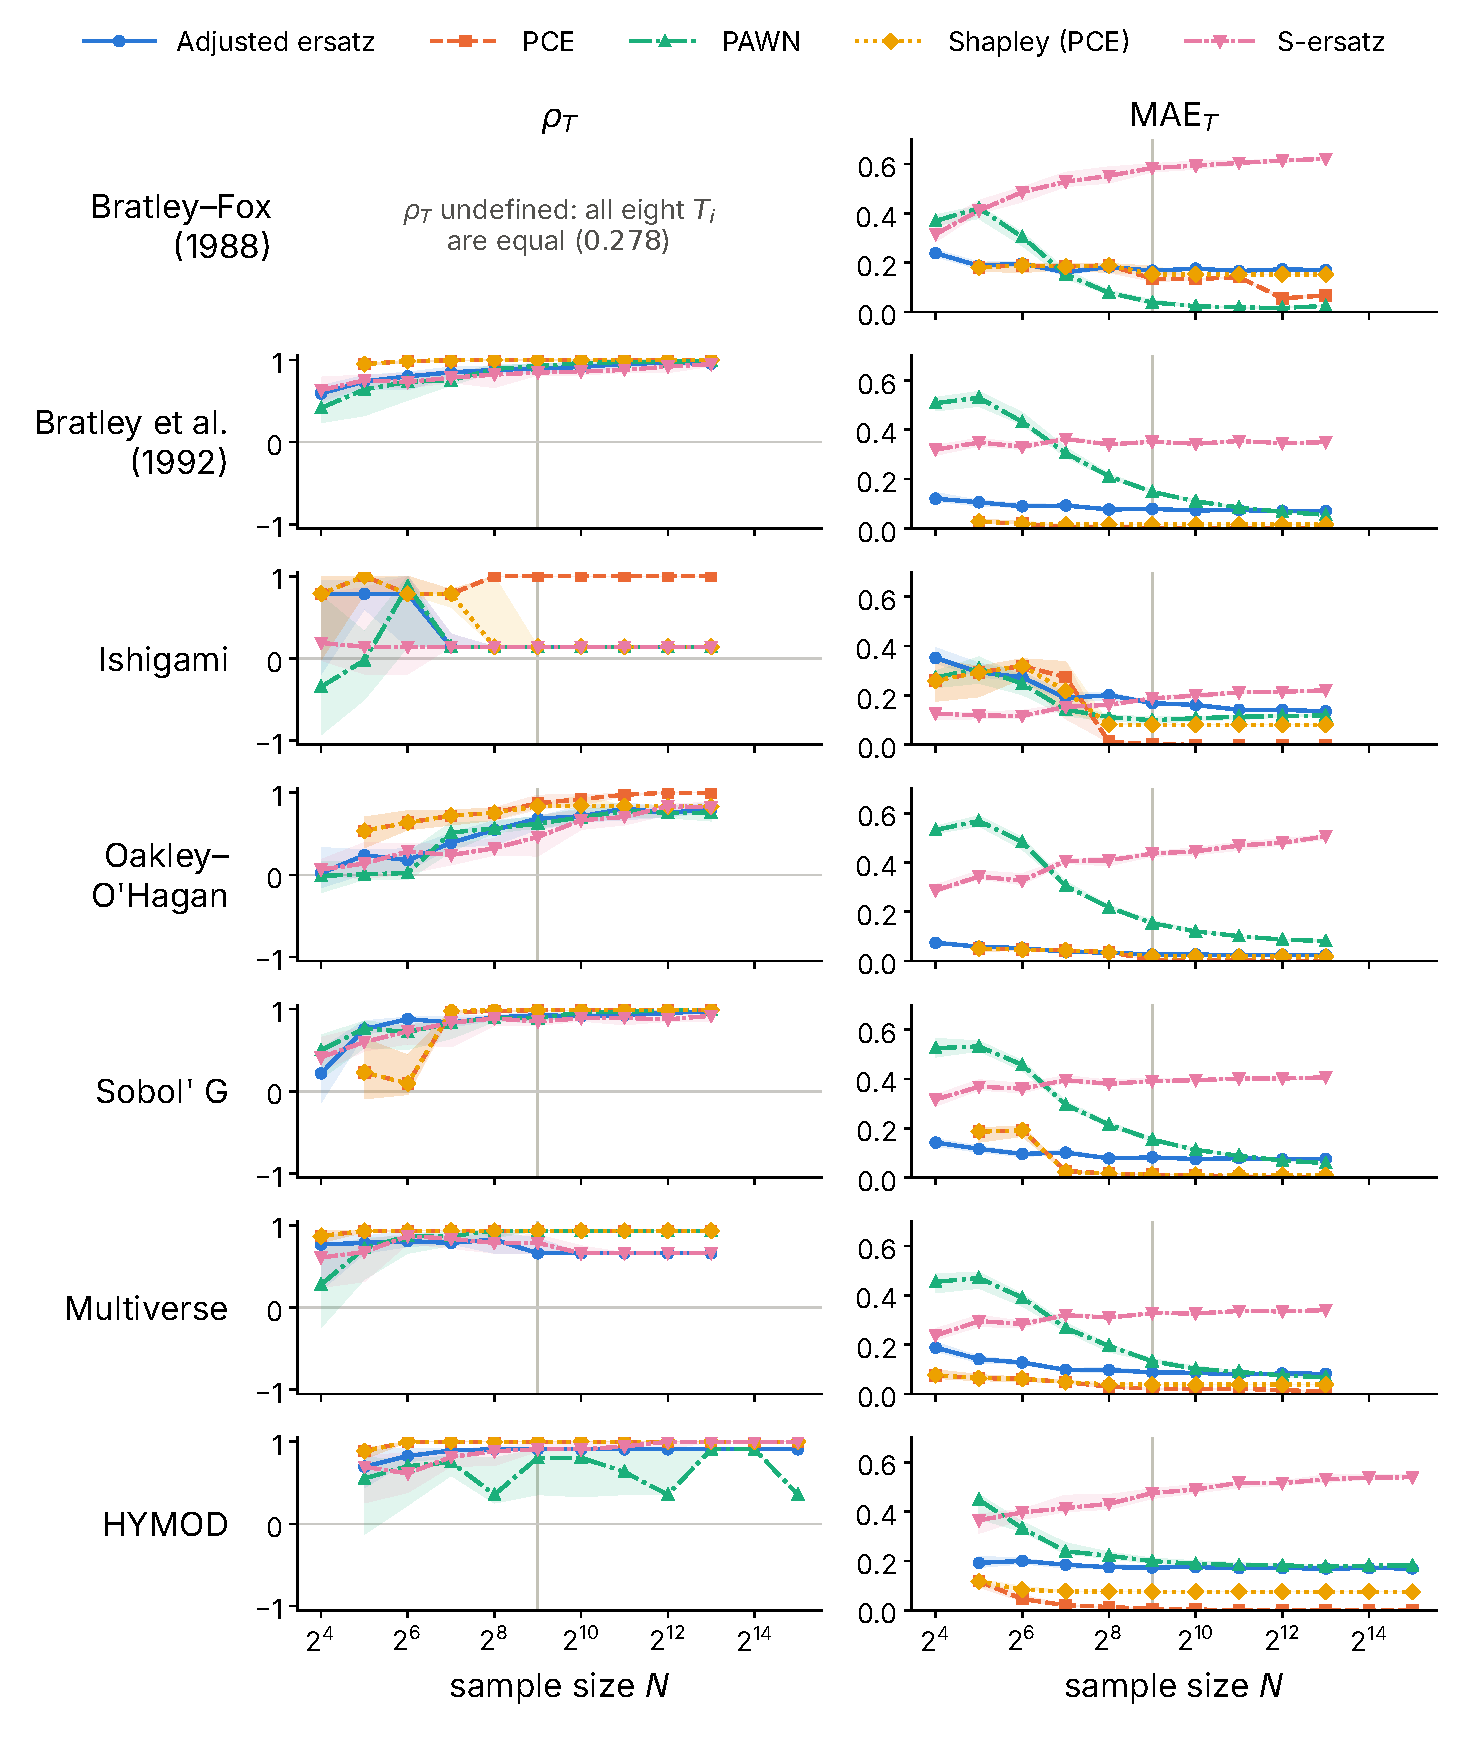
\includegraphics[width=\textwidth,height=0.85\textheight,keepaspectratio]{ris/figS_convergence_srs.pdf}
\caption{As Figure~6 of the main text, for simple random sampling (HYMOD: random subsets of the $50{,}000$ runs).}
\label{fig:conv_srs}
\end{figure}

\section*{B.6 Sensitivity analysis of the method}

\begin{table}[H]\centering\footnotesize
\begin{tabular}{@{}llcccc@{}}\toprule
Parameter & Index & $\rho_T$ & MAE$_T$ & $\alpha$ & $\beta$\\
\midrule
\multicolumn{6}{@{}l}{Adjusted ersatz}\\\addlinespace[2pt]
Grid exponent $\alpha_g$ & $S_i$ & 0.65 {\scriptsize[0.57, 0.74]} & 0.80 {\scriptsize[0.75, 0.86]} & 0.78 {\scriptsize[0.74, 0.81]} & 0.82 {\scriptsize[0.78, 0.86]}\\
 & $T_i$ & 0.92 {\scriptsize[0.86, 0.99]} & 0.92 {\scriptsize[0.88, 0.96]} & 0.93 {\scriptsize[0.90, 0.96]} & 0.91 {\scriptsize[0.87, 0.95]}\\
Fill threshold $\theta_f$ & $S_i$ & 0.09 {\scriptsize[0.06, 0.11]} & 0.08 {\scriptsize[0.06, 0.10]} & 0.05 {\scriptsize[0.04, 0.07]} & 0.08 {\scriptsize[0.07, 0.10]}\\
 & $T_i$ & 0.35 {\scriptsize[0.32, 0.38]} & 0.20 {\scriptsize[0.18, 0.21]} & 0.20 {\scriptsize[0.18, 0.21]} & 0.17 {\scriptsize[0.15, 0.18]}\\
PAWN intervals $n$ & & n/a & n/a & n/a & n/a\\
Screening threshold $\theta$ & $S_i$ & n/a & n/a & 0.02 {\scriptsize[0.01, 0.02]} & 0.01 {\scriptsize[0.01, 0.02]}\\
 & $T_i$ & n/a & n/a & 0.05 {\scriptsize[0.04, 0.05]} & 0.02 {\scriptsize[0.02, 0.02]}\\
Sampling design & $S_i$ & 0.00 {\scriptsize[0.00, 0.01]} & 0.00 {\scriptsize[0.00, 0.00]} & 0.00 {\scriptsize[0.00, 0.00]} & 0.00 {\scriptsize[0.00, 0.01]}\\
 & $T_i$ & 0.01 {\scriptsize[0.01, 0.02]} & 0.00 {\scriptsize[0.00, 0.00]} & 0.01 {\scriptsize[0.01, 0.01]} & 0.01 {\scriptsize[0.01, 0.01]}\\
\midrule
\multicolumn{6}{@{}l}{PAWN}\\\addlinespace[2pt]
Grid exponent $\alpha_g$ & & n/a & n/a & n/a & n/a\\
Fill threshold $\theta_f$ & & n/a & n/a & n/a & n/a\\
PAWN intervals $n$ & $S_i$ & 0.42 {\scriptsize[0.38, 0.45]} & 0.86 {\scriptsize[0.82, 0.91]} & 0.27 {\scriptsize[0.21, 0.35]} & --\\
 & $T_i$ & 0.47 {\scriptsize[0.45, 0.50]} & 0.87 {\scriptsize[0.84, 0.91]} & 0.74 {\scriptsize[0.66, 0.84]} & --\\
Screening threshold $\theta$ & $S_i$ & n/a & n/a & 0.16 {\scriptsize[0.12, 0.22]} & --\\
 & $T_i$ & n/a & n/a & 0.63 {\scriptsize[0.56, 0.73]} & --\\
Sampling design & $S_i$ & 0.53 {\scriptsize[0.49, 0.56]} & 0.12 {\scriptsize[0.11, 0.14]} & 0.04 {\scriptsize[0.02, 0.07]} & --\\
 & $T_i$ & 0.59 {\scriptsize[0.56, 0.62]} & 0.14 {\scriptsize[0.13, 0.15]} & 0.23 {\scriptsize[0.20, 0.26]} & --\\
\bottomrule\end{tabular}
\caption{First-order ($S_i$) and total-order ($T_i$) indices of the five algorithmic parameters with 95\% bootstrap intervals (500 resamples of the rows of the design). Scrambled Sobol' design of base size $2^{12}$ with the matrices $\mathbf A$, $\mathbf B$ and $\mathbf A_{\mathbf B}^{(i)}$, $i=1,\dots,5$ ($28{,}672$ evaluations); $S_i$ from the estimator of Saltelli et al. (2010) applied to the centred output, $T_i$ from the estimator of Jansen (1999). The difference $T_i-S_i$ is the contribution of the interactions of the parameter. n/a: the parameter does not enter the metric. --: the type~II error of PAWN is zero in 96\% of the evaluations (maximum $0.017$), so its indices are not reported.}
\label{tab:sos}
\end{table}

Figure~\ref{fig:sos_conv} shows how the indices of Table~\ref{tab:sos} change with the base size $N$. The first $N$ rows of each matrix of the design of base size $2^{12}$ form a scrambled Sobol' design of base size $N$, so the indices for $N=2^6,\dots,2^{12}$ are computed on nested designs without further model runs. Sarrazin et al.\ (2016) assess the convergence of the ranking, of the screening and of the values of the indices separately, each with a statistic computed from bootstrap resamples. Their ranking statistic, the 95\% quantile, over pairs of resamples, of a rank distance weighted by the squared indices, is zero for every metric at $N=2^{12}$, for $S_i$ as for $T_i$. For $T_i$ it is below their threshold of one from $N=2^9$ on, and the ranking by $T_i$ is the same for every metric from $N=2^7$ on. For the type~I error of PAWN the intervals of $T_i$ for $n$ ($0.74$) and $\theta$ ($0.63$) overlap, but $n$ has the larger $T_i$ in more than 99\% of the resamples. The screening statistic, the widest interval among the parameters with $T_i<0.05$ (the sampling design and the screening threshold on the metrics of the adjusted ersatz), is $0.018$ at $N=2^{12}$, below their threshold of $0.05$. The statistic for the values, the widest interval among all parameters, is $0.18$. It decreases roughly as $N^{-1/2}$, so a base size of about $2^{16}$ would be needed to bring it below $0.05$. Between $N=2^{11}$ and $N=2^{12}$ the largest changes are $0.015$ for $T_i$ and $0.023$ for $S_i$. At the present width the second decimal of the indices of the grid exponent is uncertain, but none of the conclusions of Section~3.4 of the main text depends on it.

\begin{figure}[H]
\centering
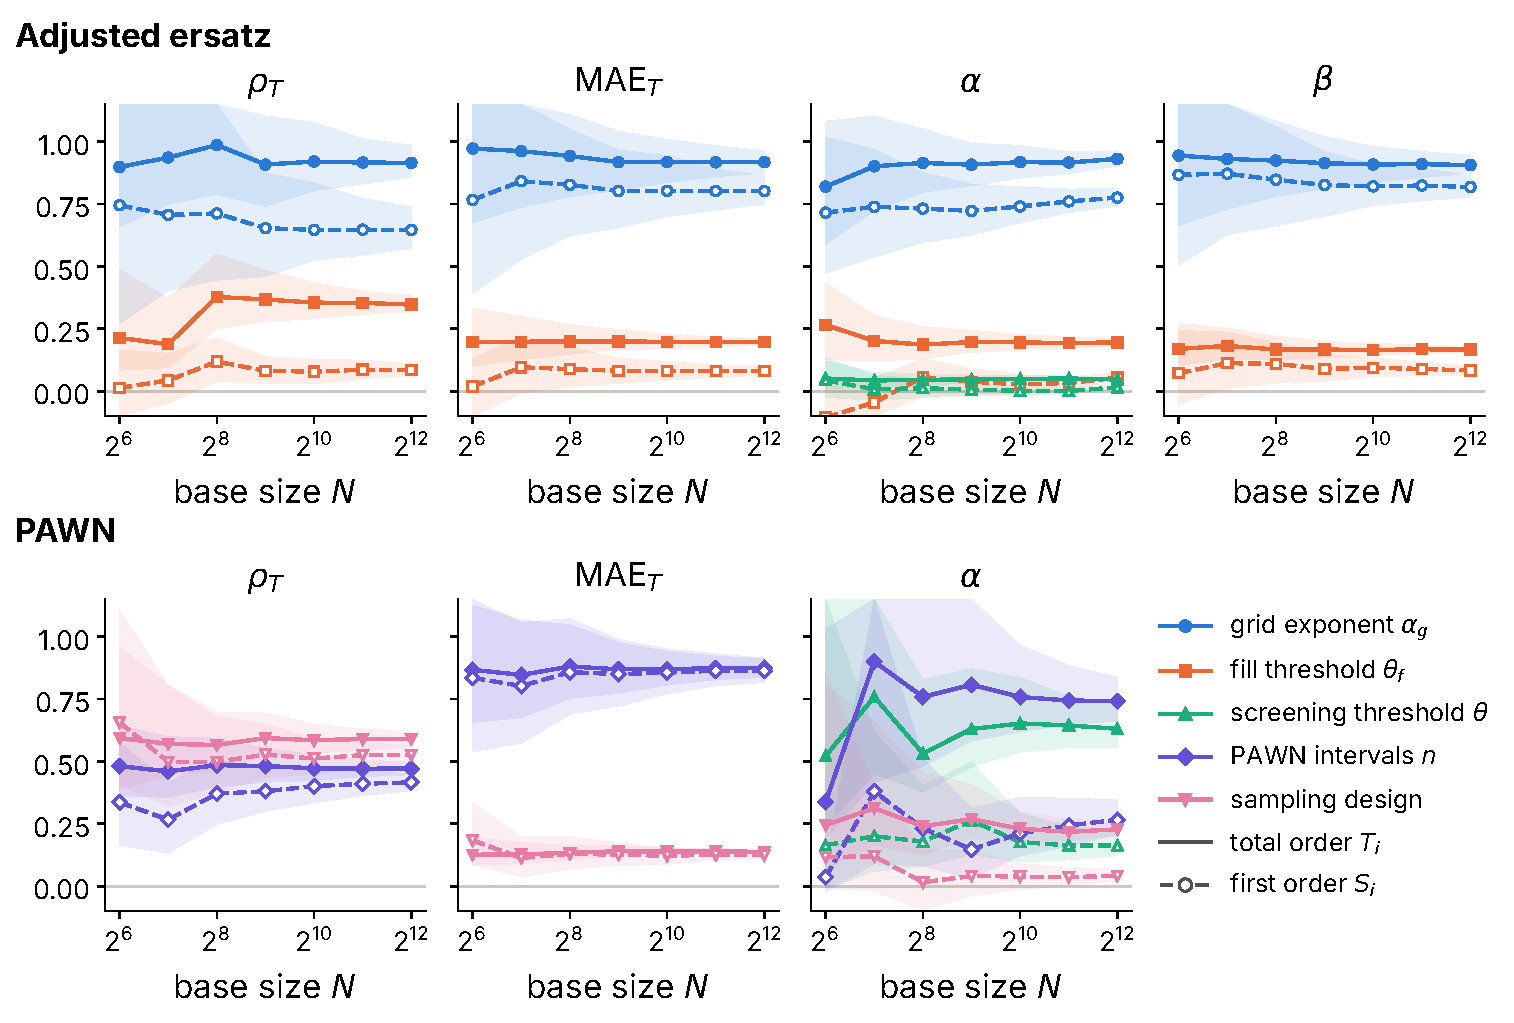
\includegraphics[width=\textwidth]{ris/figS_sos_convergence.pdf}
\caption{Indices of the algorithmic parameters as functions of the base size $N$ of the nested designs, $N=2^6,\dots,2^{12}$. Solid lines and filled markers: total-order indices $T_i$; dashed lines and open markers: first-order indices $S_i$; bands: 95\% bootstrap intervals. Parameters with $T_i<0.03$ at $N=2^{12}$ (the sampling design for the adjusted ersatz, and the screening threshold for its type~II error) are not shown, nor is the type~II error of PAWN (Table~\ref{tab:sos}).}
\label{fig:sos_conv}
\end{figure}


\section*{B.7 Screening errors and the theory}

The script \path{screening_check.py} of the repository compares the screening errors of the adjusted ersatz with the theory of Supplementary Material A. The theory covers SRS, and under SRS the two agree.

\paragraph{Limits.} For the 47 inputs of the six benchmark functions, the limit $\Psi_\lambda(C_i)$ was estimated under SRS at $\lambda=512/529$, the value of $N/s^2$ at $N=512$ ($N=61{,}952$, $s=253$), and at $\lambda=1$ ($N=65{,}536$, $s=256$), each with 10 replicates (standard errors at most $0.0011$). All 47 limits lie within the bounds $[\delta_i-\varepsilon_\lambda,\ \delta_i+\kappa_\lambda]$ of Supplementary Material A, Proposition~5.4 ($\varepsilon=0.1208$ and $\kappa=0.0548$ at $\lambda=512/529$, $\varepsilon=0.1400$ and $\kappa=0.0471$ at $\lambda=1$). The difference $\Psi_\lambda(C_i)-\delta_i$ ranges from $-0.032$ to $0.048$ at $\lambda=512/529$ and from $-0.039$ to $0.041$ at $\lambda=1$. It is largest for inputs almost independent of the output, whose limit is close to $\kappa_\lambda$, and smallest for inputs with $\delta_i$ between $0.18$ and $0.43$. The inputs missed at $\theta=0.10$ under SRS (Table~\ref{tab:scr_srs}) are those whose limit exceeds the threshold by less than about one standard deviation of the statistic at $N=512$ ($0.017$ to $0.022$): the eight inputs of the Bratley--Fox function (limit $0.113$), $x_1$ to $x_3$ of the Multiverse function ($0.117$), and $x_{11}$, $x_{13}$ and $x_{14}$ of the Oakley--O'Hagan function ($0.108$).

\paragraph{Inputs independent of the output.} The 345 inputs of the Becker ensemble with $T_i=0$ are independent of the output (main text, Proposition~3(a)), so under SRS their statistic has the distribution under independence at their sample size, whatever the model (Supplementary Material A, Theorem~4.1). Table~\ref{tab:scr_theory}(a) compares their flag rates with this distribution, simulated with 3000 replicates at each sample size. Under SRS the two agree within one standard error at the three thresholds. The maximin LHS and Sobol' designs give lower values (Supplementary Material A, Section~8 and Table~2).

\paragraph{Sample size.} Table~\ref{tab:scr_theory}(b) shows the type~I error at $\theta=0.05$ in the convergence study under SRS, together with the probability that an independent input exceeds $0.05$ (Supplementary Material A, Table~2). The type~I error oscillates with $N/s^2$ as this probability does: it is high at $N=128$, $512$ and $2048$, where $\kappa_{N/s^2}>0.05$, and low at $N=64$, $256$, $1024$ and $4096$, where $\kappa_1=0.0471<0.05$. For the Bratley et al.\ (1992) function, whose non-influential inputs have $\delta_i\le0.04$, it stays within $0.08$ of the probability for an independent input. For the Oakley--O'Hagan function it lies above that probability at every $N$, by up to $0.37$, because the limits of most of its non-influential inputs exceed $0.05$. A fixed threshold on the scale of $T_i$ therefore does not give vanishing type~I errors as $N$ grows: a consistent test needs a threshold above $\kappa_\lambda$ (Supplementary Material A, Corollary~4.5).

\paragraph{Ranking.} The 23 pairs of benchmark inputs whose $\delta_i$ differ by more than $\varepsilon_\lambda+\kappa_\lambda=0.1755$ at $\lambda=512/529$ are ranked as by $\delta$ in all 100 replicates at $N=512$ under SRS and maximin LHS, and in 99.8\% of them under the Sobol' design. The 19 pairs whose $\delta_i$ differ by more than $0.19$, the margin for $\lambda=1$ quoted in the main text, are ranked as by $\delta$ in every replicate of the three designs.

\paragraph{Designs.} At $N=512$ the maximin LHS and Sobol' designs lower the statistic of influential and non-influential inputs alike, relative to SRS: by $0.001$ to $0.014$ under maximin LHS, and by up to $0.058$ under the Sobol' design (median over the inputs of a function from $0.014$ to $0.040$; only $x_8$ of the Sobol' $G$ function is not lowered). The Sobol' design lowers it most for the functions dominated by few inputs (Bratley et al.\ 1992, Multiverse, Sobol' $G$), as for the first coordinates of the sequence (Supplementary Material A, Section~8). This causes the type~II errors of the Bratley et al.\ (1992) function in Table~\ref{tab:scr_sobol}: the means of $x_2$ and $x_3$ are $0.083$ and $0.026$ under the Sobol' design, against $0.141$ and $0.077$ under SRS. Beyond independence under plain LHS (Supplementary Material A, Proposition~8.1), the theory does not cover these designs.

\begin{table}[H]\centering\footnotesize
\begin{tabular}{@{}lcccc@{}}\toprule
\multicolumn{5}{@{}l}{(a) Becker inputs with $T_i=0$: share above $\theta$, and mean} \\
Design & $\theta=0.01$ & $\theta=0.05$ & $\theta=0.10$ & Mean \\ \midrule
SRS & 0.997 & 0.617 & 0.026 & 0.0559 \\
Maximin LHS & 0.983 & 0.359 & 0.003 & 0.0466 \\
Scrambled Sobol' & 0.942 & 0.151 & 0.003 & 0.0345 \\
\addlinespace[2pt]
Independent input, SRS, same $N$ & 0.997 & 0.608 & 0.025 & 0.0562 \\
\bottomrule\end{tabular}

\vspace{8pt}

\begin{tabular}{@{}rccccc@{}}\toprule
\multicolumn{6}{@{}l}{(b) Type~I error at $\theta=0.05$, SRS, convergence study} \\
$N$ & $N/s^2$ & Bratley et al. (1992) & Oakley--O'Hagan & Sobol' $G$ & Independent input \\ \midrule
32 & 0.889 & 0.59 & 0.57 & 0.51 & 0.57 \\
64 & 1.000 & 0.36 & 0.36 & 0.28 & 0.33 \\
128 & 0.889 & 0.79 & 0.78 & 0.77 & 0.72 \\
256 & 1.000 & 0.37 & 0.66 & 0.43 & 0.41 \\
512 & 0.968 & 0.59 & 0.75 & 0.65 & 0.57 \\
1024 & 1.000 & 0.35 & 0.54 & 0.49 & 0.35 \\
2048 & 0.968 & 0.77 & 0.91 & 0.80 & 0.71 \\
4096 & 1.000 & 0.34 & 0.64 & 0.47 & 0.27 \\
8192 & 0.989 & 0.50 & 0.94 & 0.59 & -- \\
\bottomrule\end{tabular}
\caption{Screening errors of the adjusted ersatz and the theory. (a) Inputs of the Becker ensemble with $T_i=0$ (345 for each design): share of the statistic above $\theta$, and its mean, with the same quantities for an input independent of the output under SRS at the same sample sizes (3000 replicates at each $N$). Standard errors of the observed shares: at most $0.026$. (b) Type~I error at $\theta=0.05$ in the convergence study under SRS (mean over 20 replicates), and probability that an input independent of the output exceeds $0.05$ (Supplementary Material A, Table~2; 10{,}000 replicates).}
\label{tab:scr_theory}
\end{table}

\end{document}
